\documentclass[12pt, a4paper]{article}
\usepackage{caption}
\usepackage{graphicx}
\usepackage{svg}
\usepackage{listings}
\usepackage{siunitx}
\usepackage{hyperref}
\def\checkmark{\tikz\fill[scale=0.4](0,.35) -- (.25,0) -- (1,.7) -- (.25,.15) -- cycle;}
\usepackage{tikz-network}
\hypersetup{
    colorlinks,
    citecolor=black,
    filecolor=black,
    linkcolor=black,
    urlcolor=black
}
\usepackage{amsmath, amsfonts, amssymb, amsthm}
\renewcommand{\thesubsubsection}{\thesubsection.\alph{subsubsection}}

	\usepackage{fancyhdr}
		\pagestyle{fancy}
		\setlength{\headheight}{15pt}
	\fancyhead[L]{Kristoffer Fischer Klokker}
	\fancyhead[C]{Database}
	\fancyhead[R]{6-7/5/2022}
	

\usepackage{xcolor,listings}
\usepackage{textcomp}
\usepackage{color}
\usepackage{listings}
\definecolor{codegreen}{rgb}{0,0.6,0}
\definecolor{codegray}{rgb}{0.5,0.5,0.5}
\definecolor{codepurple}{HTML}{C42043}
\definecolor{backcolour}{HTML}{F2F2F2}
\definecolor{bookColor}{cmyk}{0,0,0,0.90}  
\color{bookColor}

\lstset{upquote=true}

\lstdefinestyle{mystyle}{
    backgroundcolor=\color{backcolour},   
    commentstyle=\color{codegreen},
    keywordstyle=\color{codepurple},
    numberstyle=\numberstyle,
    stringstyle=\color{codepurple},
    basicstyle=\footnotesize\ttfamily,
    breakatwhitespace=false,
    breaklines=true,
    captionpos=b,
    keepspaces=true,
    numbers=left,
    numbersep=10pt,
    showspaces=false,
    showstringspaces=false,
    showtabs=false,
    tabsize=3,
}
\lstset{style=mystyle}
\usepackage{zref-base}

\makeatletter
\newcounter{mylstlisting}
\newcounter{mylstlines}
\lst@AddToHook{PreSet}{
  \stepcounter{mylstlisting}
  \ifnum\mylstlines=1\relax
    \lstset{numbers=none}
  \else
    \lstset{numbers=left}
  \fi
  \setcounter{mylstlines}{0}
}
\lst@AddToHook{EveryPar}{
  \stepcounter{mylstlines}
}
\lst@AddToHook{ExitVars}{
  \begingroup
    \zref@wrapper@immediate{
      \zref@setcurrent{default}{\the\value{mylstlines}}
      \zref@labelbyprops{mylstlines\the\value{mylstlisting}}{default}
    }
  \endgroup
}

\newcommand*{\mylstlines}{
  \zref@extractdefault{mylstlines\the\value{mylstlisting}}{default}{0}
}
\makeatother


\newcommand\numberstyle[1]{
    \footnotesize
    \color{codegray}
    \ttfamily
    \ifnum#1<10 0\fi#1 |
}

\newcommand{\beginSQL}{\begin{lstlisting}[ language=SQL,
                    deletekeywords={IDENTITY},
                    deletekeywords={[2]INT},
                    morekeywords={clustered},
                    framesep=8pt,
                    xleftmargin=40pt,
                    framexleftmargin=40pt,
                    frame=tb,
                    framerule=0pt ]}

\title{Database Systems / Design and Programming\\Exam}
\date{2022}
\author{Kristoffer Fischer Klokker\\ 16/08/2002\\ krklo21}
\begin{document}
	\maketitle
	\clearpage
	\tableofcontents
	\clearpage
	\section{E/R Diagraml}
		A company wants to make a database of music.  They want the following objects modeledin their system.\\
		\begin{enumerate}
			\item \textbf{Track} having Title, Length
			\item \textbf{Album} having Title, Year, List of Tracks
			\item \textbf{Artist} having Name, Telephone Number, Email Address, and List of Albums
			\item \textbf{Concert} having Location, Date, Artist, List of Tracks
		\end{enumerate}
		They also describe the relationships between the objects.  Each track appears on one album.  Each album is produced by one artist.  Each concert is held by one artist, who plays a number of tracks from his/her albums.
		\subsection{Create  an  E/R  diagram  capturing  the  objects  and  relationships  described  above. Ensure that your model does not contain redundant information. Describe all your design choices and constraints}
			\begin{figure}[h!]
				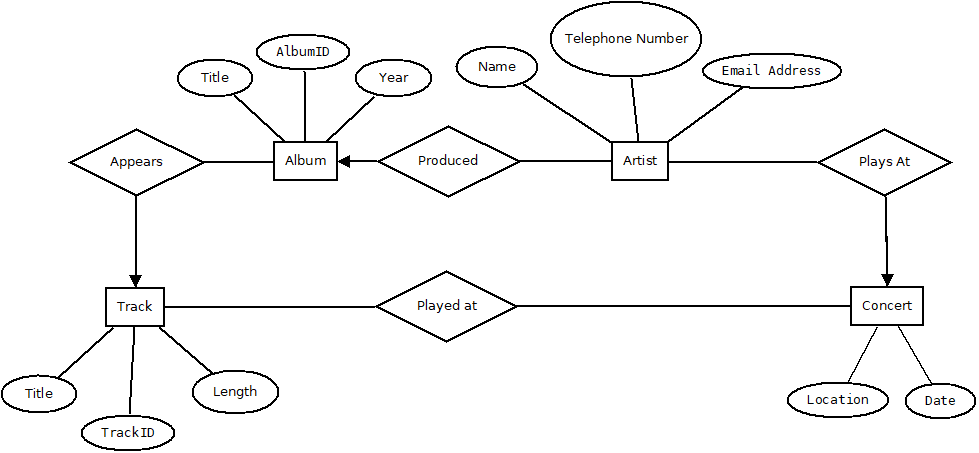
\includegraphics[width=\textwidth]{assets/ER1.png}
				\centering
				\caption{E/R model with relations and objects}
			\end{figure}
			For the the relation Appears from Track to Album, a many one relation is made and the List of Tracks is therefore not needed.\\
			The relation Produced is also many one and eleminate the need for List of Albums on an artist.\\
			Plays at is also a many one relation due to the text describing only one artist being able to play at an concert.\\
			The concert also has a relation Played at, from track to concert. This relation was described as tracks from the artists album, but if the relation should be at the album the whole album needed to be played. Therefore it is a many many relation between track and concert.
		\subsection{For  each  entity  set,  determine  an  appropriate  key  and  underline  it.  If you feel the attributes of an entity set do not form an appropriate key, you are allowed to introduce an ID. }
			\begin{figure}[h!]
				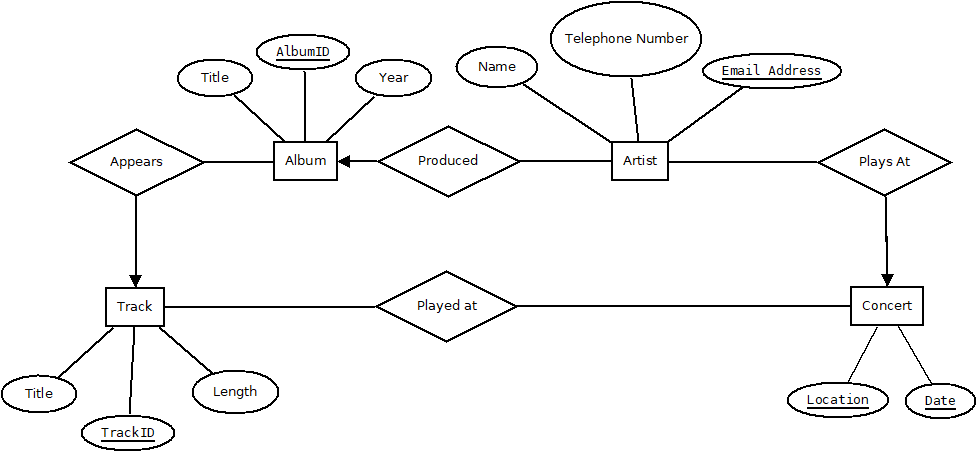
\includegraphics[width=\textwidth]{assets/ER2.png}
				\centering
				\caption{Figure 1 but with keys for the objects}
			\end{figure}
			For Album I choose to create a unique ID, due to an artist may revise and rerelease an album the same year.\\
			The same goes for a track, it may be remixed or revised, so a unique ID is also required.\\
			For the artist the Email Address can be used, due to it already being unique. The only problem may be if the artist have a personal and a business email, but that would require a whole new object. So therefore it is assumed the artist only have 1 email.\\
			The concert key is Location and Date due to no two concert can be played at the exact same address and date if time is included in date.
		\section{From E/R diagram torelational model}
			\begin{figure}[h!]
				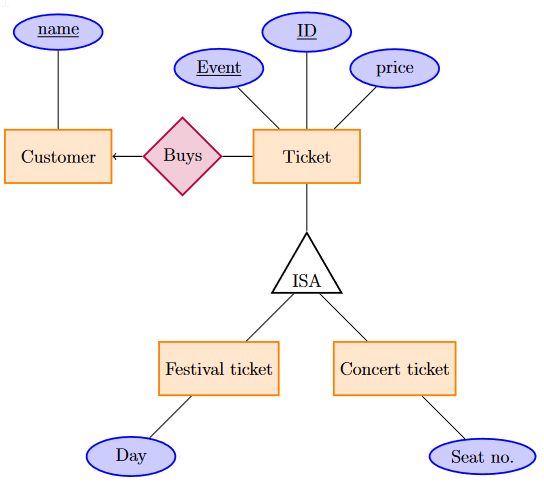
\includegraphics[width=\textwidth]{assets/ERT0.png}
				\centering
			\end{figure}
			A ticket agency has modeled their database system using the above E/R diagram. Now they need your help to translate it to relational schemata. They are unsure which translation to use and give you the following tasks.
			\subsection{The relational schemata must be created using the E/R-style translation}
				Ticket(\underline{Event},\underline{ID},price)\\
				Customer(\underline{name})\\
				Buys(\underline{name},\underline{Event},\underline{ID})\\
				FestivalTicket(\underline{Event},\underline{ID},day)\\
				ConcertTicket(\underline{Event},\underline{ID},Seat no.)
			\subsection{The relational schemata must be created using the object-oriented translation}
				Ticket(\underline{Event},\underline{ID},price)\\
				Customer(\underline{name})\\
				Buys(\underline{name},\underline{Event},\underline{ID})\\
				Festival ticket(\underline{Event},\underline{ID},price,day)\\
				ConcertTicket(\underline{Event},\underline{ID},price,Seat no.)\\
				ConcertFestivalTicket(\underline{Event},\underline{ID},price,Seat no., Day)
			\subsection{The relational schemata must be created using the null translation}
				Ticket(\underline{Event},\underline{ID},price,Day,Seat no.)\\
				Customer(\underline{name})\\
				Buys(\underline{name},\underline{Event},\underline{ID})\\
				The buys relation still has to be its own relation, due to the customer may buy ticket for different event and thus create redundencies.
			\subsection{Write CREATE TABLE statements for the second translation (b), namely for the object-oriented translation}
				\beginSQL
CREATE TABLE Ticket(
	Event VARCHAR(40),
	ID INT,
	Price FLOAT,
	PRIMARY KEY(Event,ID)
);
CREATE TABLE Customer(
	Name VARCHAR(40) PRIMARY KEY
);
CREATE TABLE Buys(
	Name VARCHAR(40) REFERENCES Customer(Name),
	Event VARCHAR(40) REFERENCES Ticket(Event),
	ID INT REFERENCES Ticket(ID)
);
CREATE TABLE FestivalTicket(
	Event VARCHAR(40) REFERENCES Ticket(Event),
	ID INT REFERENCES Ticket(ID),
	Price FLOAT,
	Day DATE,
	PRIMARY KEY(Event,ID)
);
CREATE TABLE ConcertTicket(
	Event VARCHAR(40) REFERENCES Ticket(Event),
	ID INT REFERENCES Ticket(ID),
	Price FLOAT,
	SeatNo INT,
	PRIMARY KEY(Event,ID)
);
CREATE TABLE ConcertFestivalTicket(
	Event VARCHAR(40) REFERENCES Ticket(Event),
	ID INT REFERENCES Ticket(ID),
	Price FLOAT,
	SeatNo INT,
	Day DATE,
	PRIMARY KEY(Event,ID)
);\end{lstlisting}
	For the ISA object, the keys have been choosen to be references to Ticket relation.
	\clearpage
	\section{SQL queries}
	\begin{figure}[h!]
		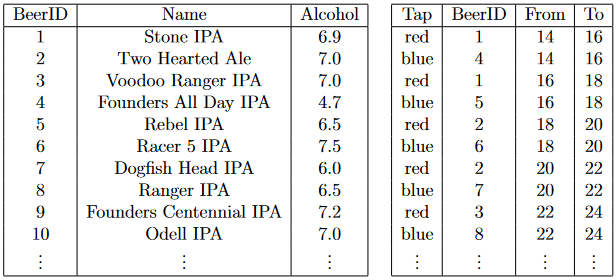
\includegraphics[width=\textwidth]{assets/sql.png}
		\centering
		\caption{To the left, tablebeers.  To the right, tabletaps.}
	\end{figure}
	This task is set in a pub specialising in Indian Pale Ales (IPAs).  The pub has far more kegs of IPAs than taps to connect them to. Thus, each kegs is at most connected to a tap some of the time.  To keep track of this and to inform the customers, the pub maintains a database system.\\
	Figure 3 shows the schemas and some example data for two important tables of the database.  The left table,beers,  contains information about the beers available. Each beer has a unique numeric BeerID. It also has a name and its alcohol percentage.\\
	The right table,taps,  contains information about which beer (keg) is connected to which tap at what time. The left-most column shows the name of tap, the second the numeric id of the beer connected between the two times specified in the third and fourth column.  Not all taps have to have a beer connected and not all beers need to be connected to a tap.\\
	In the following tasks, you should write a single SQL expression.
	
		\subsection{Write an SQL SELECT query without subqueries, which lists the names of all beers that are served from at least one tap Only those names should occur, and they should only occur once}
			\beginSQL
SELECT DISTINCT Name FROM beers, taps WHERE beers.BeerID = taps.BeerID\end{lstlisting}
		\subsection{Write an SQL SELECT query with subqueries, which lists the alcohol percentages served from the red tap for all beers that have the string “IPA” as a substring.}
			\beginSQL
SELECT Alcohol FROM beers WHERE beers.BeerID IN(SELECT BeerID FROM taps WHERE Tap = 'red') AND Name Like '\%IPA\%'\end{lstlisting}
		\subsection{Write an SQL SELECT query, which lists all taps together with the average alcohol percentage of the beers that they are connected to. There should be exactly one row for each tap in the result. If a beer is connected to a tap multiple times per day, it should contribute only once}
			\beginSQL
SELECT Tap,AVG(Alcohol) FROM 
(SELECT DISTINCT BeerID,Tap FROM taps) AS DisBeer,
beers WHERE DisBeer.BeerID = beers.BeerID GROUP BY Tap\end{lstlisting}
	\clearpage
	\section{Relational algebra}
		\subsection{For each of the following expressions, give the resulting relation as a table similar to the ones for R and S above.}
			
			\begin{minipage}{0.45\textwidth}
			\centering	
			\begin{tabular}{|l|l|l|}
			\hline
			A & B  & C \\ \hline
			1 & 2 & 3 \\ \hline
			9 & 8 & 3 \\ \hline
			4 & 7 & 1 \\ \hline
			\end{tabular}\\[4mm]
			R
			\end{minipage}
			\begin{minipage}{0.45\textwidth}
			\centering	
			\begin{tabular}{|l|l|l|}
			\hline
			A & B & D \\ \hline
			2 & 3 & 1\\ \hline
			3 & 1 & 3\\ \hline
			4 & 7 & 9\\ \hline
			\end{tabular}\\[4mm]
			S
			\end{minipage}
			\subsubsection{$\sigma_{C>D}(\sigma_{R.A<S.A}(R\times S))$}
				\begin{table}[h!]
				\begin{tabular}{|l|l|l|l|l|l|}
				\hline
				R.A & R.B & C & S.A & S.B & D \\ \hline
				1 & 2 & 3 & 2 & 3 & 1\\ \hline
				\end{tabular}
				\end{table}
			\subsubsection{$\Pi_{A,B}(S)\cap \Pi_{C,A}(R)$}
				\begin{table}[h!]
				\begin{tabular}{|l|l|}
				\hline
				A & B \\ \hline
				2 & 3\\ \hline
				4 & 7\\ \hline
				\end{tabular}
				\end{table}
			\subsubsection{$\gamma_{C,sum(A)}(R)$}
				\begin{table}[h!]
				\begin{tabular}{|l|l|}
				\hline
				C & SUM(A) \\ \hline
				3 & 10\\ \hline
				1 & 4\\ \hline
				\end{tabular}
				\end{table}
			\subsubsection{$\sigma_{A>D}(S)$}
				\begin{table}[h!]
				\begin{tabular}{|l|l|l|}
				\hline
				A & B & D \\ \hline
				2 & 3 & 1\\ \hline
				\end{tabular}
				\end{table}
			\clearpage
			\subsubsection{$R\bowtie S$}
				\begin{table}[h!]
				\begin{tabular}{|l|l|l|l|}
				\hline
				A & B & C & D \\ \hline
				4 & 7 & 1 & 9\\ \hline
				\end{tabular}
				\end{table}
		\subsection{For each of the following SQL statements, write an expression of extended relational algebra which is equivalent in its effect to the following SQL statement independent of the actual tuples present in R and S}
			\subsubsection{SELECT R.B,S.A,D,C FROM S JOIN R ON R.B=S.B AND C $>$ D}
				$\sigma_{R.B,S.A,D,C}(S\bowtie_{R.B=S.B\land C>D}R)$
			\subsubsection{SELECT DISTINCT D, avg(A) FROM S WHERE D= 4 OR B= 2 GROUP BY D}
				$\gamma_{D,AVG(A)}(\sigma_{D=4\lor B=2}(S))$\\
				The distinct part of the query is not needed, due to the grouping, which will not result in any possible duplicates.
	\clearpage
	\section{Normalization}
		Consider the relation
			$$R(SenderID,SenderName,ReceiverID, ReceiverName, External, Message, Hash)$$
		with the following functional dependencies:
		\begin{enumerate}
			\item $SenderID\rightarrow SenderName$
			\item $ReceiverID \rightarrow ReceiverName$
			\item $SenderID\;ReceiverID \rightarrow External$
			\item $Message \rightarrow Hash$
			\item $SenderID\;ReceiverID\;Hash\rightarrow Message$
		\end{enumerate}
		\subsection{List all keys of R and argue why there can be no other keys}
			There are two possible keys:\\
			$\{SenderID,ReceiverID,Message\}$\\
			$\{SenderID,ReceiverID,Hash\}$\\
			Superkeys are possible from these, but only two keys are possible due to the rest of the attributes are on the rightside of the FD's
		\subsection{Analyze whether R is BCNF. If it is, show that there are no BCNF violations. If it is not, show that there is at least one BCNF violation and decompose R until it is in BCNF}
			The first violation is $SenderID\rightarrow SenderName$\\
			$R_1=SenderID^+=\{SenderName,SenderID\}$\\
			$R_2=R-(SenderID^+-SenderID)$\\
			$R_2=\{SenderID,ReceiverID, ReceiverName, External, Message, Hash\}$\\
			Where $R_1$ has the FD $SenderID\rightarrow SenderName$ and is in BCNF now\\
			And $R_2$ is not BCNF due to $ReceiverID \rightarrow ReceiverName$\\[4mm]
			
			The decomposition is just like for $R_1$ and $R_2$ but with receiver resulting in:\\
			$R_3=ReceiverID^+=\{ReceiverID, ReceiverName\}$\\
			$R_4=R_2-(ReceiverID^+-ReceiverID)$\\
			$R_4=\{SenderID,ReceiverID, External, Message, Hash\}$\\
			Now $R_3$ is BCNF with the FD $ReceiverID \rightarrow ReceiverName$\\
			$R_4$ is not BCNF due to the violation of $SenderID\;ReceiverID \rightarrow External$\\[4mm]
			
			$R_5=\{SenderID,ReceiverID\}^+=\{SenderID,ReceiverID,External\}$\\
			$R_6=R_4-(\{SenderID,ReceiverID\}^+-\{SenderID,ReceiverID\})$\\
			$R_6=\{SenderID,ReceiverID, Message, Hash\}$\\
			$R_5$ is BCNF with the FD $SenderID\;ReceiverID\;Hash\rightarrow Message$\\
			While $R_6$ is not BCNF due to  $Message \rightarrow Hash$\\[4mm]
			
			$R_7=Message^+=\{Message,Hash\}$\\
			$R_8=R_6-(Message^+-Message)=\{SenderID,ReceiverID, Message\}$\\
			$R_7$ is BCNF with the FD $Message \rightarrow Hash$\\
			$R_8$ is BCNF with no FD\\[4mm]
			Therefore the final relation is:\\
			$R_1=\{SenderName,SenderID\}$\\
			$R_3=\{ReceiverID, ReceiverName\}$\\
			$R_5=\{SenderID,ReceiverID,External\}$\\
			$R_7=\{Message,Hash\}$\\
			$R_8=\{SenderID,ReceiverID, Message \}$\\
		\subsection{What would change if we would consider 3NF instead of BCNF? Explain your answer}
			It would result in $R_6$ not getting decomposed. This is due to $R_6$  having the FD's:\\
			$Message \rightarrow Hash$\\
			$SenderID\;ReceiverID\;Hash\rightarrow Message$\\
			BCNF would not allow the first FD, but in 3NF it is allowed due to $Hash$ being part of a key. The other FD is allowed due to the left side being a superkey.
\end{document}


